% journal.tex
% Template file to use for LLNCS papers prepared in LaTeX
% websites for more information: http://www.springer.com
%http://www.springer.com/lncs

\documentclass{llncs}
\usepackage{setspace}
\usepackage[bahasa]{babel}
\usepackage{graphicx}
%Use this line instead if you want to use running heads (i.e. headers on each page):
%\documentclass[runningheads]{llncs}

\begin{document}
\title{Analisa Unjuk Kerja Format Serialisasi Data JSON dan XML}

%If you're using runningheads you can add an abreviated title for the running head on odd pages using the following
%\titlerunning{abreviated title goes here}
%and an alternative title for the table of contents:
%\toctitle{table of contents title}

%\subtitle{Subtitle Goes Here}

%For a single author
%\author{Author Name}

%For multiple authors:
\author{Muhammad Ghazali\inst{1}}


%If using runnningheads you can abbreviate the author name on even pages:
%\authorrunning{abbreviated author name}
%and you can change the author name in the table of contents
%\tocauthor{enhanced author name}

%For a single institute
%\institute{Institute Name \email{email address}}

% If authors are from different institutes 
\institute{Teknik Informatika, Fakultas Teknik, Universitas Widyatama \\Cikutra No. 204 A Bandung,
Jawa Barat, Indonesia 40124 \email{muhammad.ghazali@widyatama.ac.id}}

%to remove your email just remove '\email{email address}'
% you can also remove the thanks footnote by removing '\thanks{Thank you to...}'


\maketitle

\begin{abstract}

\onehalfspacing JSON digunakan untuk merepresentasikan data berbasis teks dalam format yang dapat dikonsumsi dengan mudah oleh aplikasi lain. Penulis memilih format serialisasi data JSON karena JSON lebih mudah ditulis dan dibaca oleh mesin (komputer) dan manusia. Selain itu JSON lebih mudah untuk diproses karena memiliki struktur yang lebih sederhana dibandingkan XML\cite{json-fat-free}\cite{json-vs-xml-debate}.

\onehalfspacing Penulis membuktikan bahwa data yang diserialisasikan dalam format JSON memiliki ukuran yang lebih kecil dibandingkan XML. Disini penulis hanya membandingkan ukuran data yang dihasilkan setelah dilakukan serialisasi. Hal tersebut dibuktikan dengan membangun purwa-rupa Web API untuk menerapkan JSON pada \textit{resource} yang akan dikonsumsi oleh aplikasi lain. Dengan membangun purwa-rupa Web API ini dibuktikan juga bahwa API yang menserialisasikan data dalam format JSON mampu melayani permintaan \textit{web resource} lebih banyak dibandingkan dengan API yang menserialisasikan data dalam format XML.

Kata kunci: Web API, JSON, Format Serialisasi Data
\end{abstract}

\section{Pendahuluan}

% menjelaskan obyek penelitian
\onehalfspacing Dalam penelitian ini penulis membahas mengenai topik menarik tentang analisa unjuk kerja format serialisasi data JSON\footnote{Lihat bagian Landasan teori: JSON} dan XML\footnote{Lihat bagian Landasan teori: XML}. Hal yang dipelajari adalah untuk membuktikan bahwa data yang diserialisasi dalam format JSON memiliki ukuran data yang lebih kecil jika dibandingkan dengan data yang diserialisasi dalam format XML. Untuk membuktikan hal tersebut penulis mengambil studi kasus implementasi Web API untuk CampusLife \textit{mobile information directory application}.

Web API\footnote{Lihat bagian Landasan teori: Web API} dibangun dengan tujuan untuk membuka akses secara tidak langsung ke \textit{data store}\footnote{http://en.wikipedia.org/wiki/Data\_store} yang tersimpan di salah satu layanan \textit{Database as a Service}\footnote{http://en.wikipedia.org/wiki/Cloud\_database} yang digunakan oleh LLM di AppFog\footnote{http://www.appfog.com/}. Seluruh data-data \textit{event} yang tersimpan di \textit{data store} akan diolah oleh Web API menjadi data dengan format yang dapat dikonsumsi dengan mudah oleh aplikasi \textit{mobile} CampusLife. Proses pengolahan tersebut dinamakan serialisasi data\footnote{Lihat bagian Landasan teori: Serialiasi Data}.

\onehalfspacing Namun, hal yang menjadi fokus di penelitian ini bukanlah tentang implementasi Web API tersebut, melainkan tentang analisa unjuk kerja dari penerapan format serialisasi data ketika data dikirimkan dari Web API ke \textit{client}. Web API hanya akan dibangun sebagai pendukung untuk membantu penulis dalam menganalisa ukuran data yang diformat JSON dan XML ketika dikirimkan ke \textit{client}. Mulai dari bab ini dengan selanjutnya data-data yang yang dikirimkan dari Web API ke \textit{client} akan sering disebut \textit{resource}. 

% Pada bagian ini jelaskan rumusan masalah yang akan diteliti
\onehalfspacing Adapun masalah yang diteliti dalam penelitian ini dapat dirumuskan sebagai berikut:
\begin{enumerate}
  \item Seberapa kecil ukuran \textit{resource} yang diformat dalam JSON jika dibandingkan dengan ukuran \textit{resource} yang diformat dalam XML? 
  \item Bagaimana implikasi terhadap jumlah permintaan  \textit{resource} yang berhasil dikembalikan oleh Web API jika \textit{resource} diformat dalam JSON dan XML?
\end{enumerate}

\section{Metodologi}
\onehalfspacing Adapun tahapan penelitian yang dilakukan oleh penulis adalah sebagai berikut:
\begin{enumerate}
  \item \textbf{Identifikasi masalah dan perumusan hipotesis}. Pada tahap ini penulis merumuskan masalah yang diteliti.
  \item \textbf{Pengujian format serialiasi JSON dan XML}. Pada tahap ini penulis melakukan pengujian serialisasi dengan membangun purwa-rupa Web API untuk mendukung proses pengujian serialiasi data dalam format JSON dan XML.
  \item \textbf{Analisis unjuk kerja serialisasi}. Pada tahap ini penulis menganalisis unjuk kerja dari format serialisasi JSON dan XML dengan melakukan beberapa skenario pengujian.
  \item \textbf{Merumuskan kesimpulan}. Pada tahap ini penulis membuat kesimpulan hasil analisis dari unjuk kerja format JSON dan XML.
\end{enumerate}

Visualisasi dari tahapan yang dijelaskan di bagian sebelumnya dapat dilihat pada gambar \ref{visualisasi-metodologi}.

\onehalfspacing
\begin{figure}[htp]
\centering
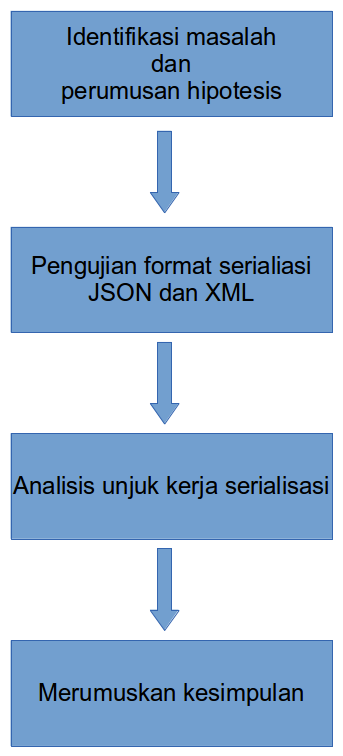
\includegraphics[scale=0.45]{images/visualisasi-metodologi.png}
\caption{Visualisasi Metodologi}
\label{visualisasi-metodologi}
\end{figure}

\section{Penutup}

\subsection{Kesimpulan}

Selama menjalani masa penelitian penulis mendapatkan beberapa kesimpulan dari hasil penerapan JSON sebagai format serialisasi data:

\begin{enumerate}
  \item Berdasarkan hasil pengujian yang sudah dilakukan, terbukti bahwa data yang diserialisasi dalam format JSON memiliki ukuran data yang lebih kecil jika dibandingkan dengan data yang diserialisasi dalam format XML.
  \item Implikasi dari penerapan JSON pada \textit{resource} adalah jumlah permintaan yang berhasil dikembalikan jauh lebih banyak dibandingkan ketika Web API mengembalikan \textit{resource} dalam format XML.
\end{enumerate}

\subsection{Saran}

Untuk mengembangkan hasil penelitian ini, penulis menyarankan beberapa topik pengembangan berikut:

\begin{enumerate}
  \item Membandingkan JSON secara eksplisit dengan beberapa format serialisasi yang lain dalam hal keunggulan dan kelemahan
  \item Melakukan pengujian Web API dengan mengaksesnya melalui aplikasi
  \item Meneliti isu-isu keamanan ketika menerapkan JSON
  \item Menganalisa trend penggunaan format serilisasi data tertentu  
  \textit{mobile}
\end{enumerate}

Demikian saran-saran yang dapat penulis sampaikan, penulis berharap laporan ini dapat bermanfaat bagi semua pihak yang membaca.

%The bibliography, done here without a bib file
%This is the old BibTeX style for use with llncs.cls
\bibliographystyle{splncs}

%Alternative bibliography styles:
%the following does the same as above except with alphabetic sorting
%\bibliographystyle{splncs_srt}
%the following is the current LNCS BibTex with alphabetic sorting
%\bibliographystyle{splncs03}
%If you want to use a different BibTex style include [oribibl] in the document class line

\begin{thebibliography}{1}
%add each reference in here like this:

\bibitem[1]{agile-samurai}
Rasmusson, Jonathan (2010) The Agile Samurai: The Pragmatic Bookshelf.

\bibitem[2]{challenging-issues-and-limitations-of-mobile-computing}
Deepak, G., and Dr. Pradeep B S. \emph{Challenging Issues and Limitations of Mobile Computing}. International Journal of Computer Technology and Applications 3.1 (2012): Academic Journals Database. Web. 8 Jan. 2013.

\bibitem[3]{comparison-of-data-serialization-formats}
Audie Sumaray dan S. Kami Makki. \emph{A comparison of data serialization formats for optimal efficiency on a mobile platform}. 6th International Conference on Ubiquitous Information Management and Communication (2012): Artikel No. 48. ACM Digital Library. Web. 24 Jan 2013

\bibitem[4]{json-vs-xml-debate}
Marinescu, Floyd dan Tilkov, Stefan. "Debate: JSON vs. XML as a data interchange format." \emph{Infoq}. Web. 20 Januari 2013. http://www.infoq.com/news/2006/12/json-vs-xml-debate

\bibitem[5]{rest-soap}
Marinescu, Floyd dan Tilkov, Stefan. "How REST replaced SOAP on the Web: What it means to you." \emph{Infoq}. Web. 11 Januari 2013. http://www.infoq.com/articles/rest-soap

\bibitem[6]{ws-restful}
Rodriguez, Alex. "RESTful Web services: The basics." \emph{IBM}. Web. 11 Januari 2013. http://www.ibm.com/developerworks/webservices/library/ws-restful/

\bibitem[7]{json-fat-free}
"JSON: The Fat-Free Alternative to XML." \emph{JSON Official Website}. Web. 20 Januari 2013. http://www.json.org/xml.html

\bibitem[8]{introducing-json}
"Introducing JSON" \emph{JSON Official Website}. Web. 20 Januari 2013. http://www.json.org/
  
\bibitem[9]{three-tier-architecture}
Ramirez, Ariel Ortiz. "Three-Tier Architecture." \emph{Linux Journal}. Web. 18 Maret 2013. http://www.linuxjournal.com/article/3508

\bibitem[10]{apis-linux-journal}
Reuven, Lerner. "APIs." \emph{Linux Journal}. Web. 18 Maret 2013. http://www.linuxjournal.com/content/apis

\bibitem[11]{json-continue-to-winning}
Irani, Romin. "JSON Continues its Winning Streak Over XML." \emph{ProgrammableWeb Blog}. Web. 8 April 2013. http://blog.programmableweb.com/2010/12/03/json-continues-its-winning-streak-over-xml/

\bibitem[12]{json-continue-to-push}
Perkins, Luc. "Why JSON will continue to push XML out of the picture." \emph{ProgrammableWeb Blog}. Web. 8 April 2013. http://blog.appfog.com/why-json-will-continue-to-push-xml-out-of-the-picture/

\bibitem[13]{rfc-4627}
Crockford, Douglas. "The application/json Media Type for JavaScript Object Notation (JSON)." \emph{RFC Index}. Web. 5 April 2013. http://tools.ietf.org/html/rfc4627
  
\bibitem[14]{agile-manifesto}
  "Manifesto Pengembangan Perangkat Lunak Agile" \emph{Agile Manifesto}. Web. 8 April 2013. http://agilemanifesto.org/iso/id/
  
\bibitem[15]{introducing-bdd}
  "Introducing BDD" \emph{Dan North \& Associates}. Web. 7 Mei 2013. http://dannorth.net/introducing-bdd/
  
\bibitem[16]{whats-in-story}
  "What's in a Story?" \emph{Dan North \& Associates}. Web. 7 Mei 2013. http://dannorth.net/whats-in-a-story/
  
\bibitem[17]{jbge-scott}
  "Just Barely Good Enough Models and Documents: An Agile Best Practice." \emph{Agile Modelling}. Web. 10 Mei 2013. http://www.agilemodeling.com/essays/barelyGoodEnough.html
  
\bibitem[18]{multitier-architecture-wikipedia}
  "Multitier architecture." \emph{Wikipedia}. Web. 15 Maret 2013. http://en.wikipedia.org/wiki/Multitier\_architecture
  
\bibitem[19]{api-wikipedia}
  "Application Programming Interface." \emph{Wikipedia}. Web. 22 Maret 2013. http://en.wikipedia.org/wiki/Application\_programming\_interface
    
\bibitem[20]{web-api}
  "Web API." \emph{Wikipedia}. Web. 20 Januari 2013. http://en.wikipedia.org/wiki/Web\_API
  
\bibitem[21]{xml-wikipedia}
  "XML." \emph{Wikipedia}. Web. 7 April 2013. http://en.wikipedia.org/wiki/XML
  
\bibitem[22]{acceptance-testing-wikipedia}
  "Acceptance Testing." \emph{Wikipedia}. Web. 7 Mei 2013. http://en.wikipedia.org/wiki/Acceptance\_testing

\bibitem[23]{serialization-wikipedia}
  "Serialization." \emph{Wikipedia}. Web. 24 Januari 2012. http://en.wikipedia.org/wiki/Serialization

\bibitem[24]{agile-wikipedia}
  "Agile software development." \emph{Wikipedia}. Web. 24 Januari 2013. http://en.wikipedia.org/wiki/Agile\_software\_development
\end{thebibliography}

\end{document}

